\documentclass[no-page-number]{nanzan-abstract}
\usepackage{url}
\usepackage{graphicx}
\usepackage{tikz}
\usepackage{array}
\usepackage{booktabs}
\usetikzlibrary{arrows.meta,positioning}
\setlength{\tabcolsep}{2.5pt}
\ModifyHeading{section}{font={\large\bfseries},format={\vbox{\noindent #1#2}},lines=2,before_space=0.8ex,after_space=0.5ex}
\AtBeginDocument{\fontsize{9.5pt}{11.3pt}\selectfont}

\title{姿勢推定を用いた筋力トレーニング評価システムにおける処理の共通化}
\author{2023TS030 川瀬 翔大}
\professor{宮澤 元}

\begin{document}
\maketitle

\section{はじめに}
筋力トレーニングでは，フォームが崩れると狙った部位に十分な負荷をかけにくくなり，トレーニングの効率低下につながる可能性がある．しかし，運動中の自分のフォームを客観的かつ継続的に確認することは難しい．そこで，カメラ映像から人体の姿勢を推定し，関節位置や角度を用いて運動フォームを評価するシステムが研究されている．このようなシステムでは，映像から得たランドマークから特徴量を計算し，あらかじめ定めた評価規則に基づいてフォームを判定できる．
\par
一方，対応する筋力トレーニング種目を増やすと，種目ごとに評価対象の関節，目標角度，許容範囲，比較条件などが異なるため，角度計算・判定・表示のコードに種目固有の条件を追加する必要が生じる．種目数が増えるほど条件分岐が増え，既存処理への影響確認も必要となるため，実装・保守の負担が大きくなる．逆にすべてを共通化すると，種目固有の評価規則を扱えない可能性がある．
\par
そこで本研究の目的を，\textbf{種目追加時に既存プログラムを修正する負担を抑えつつ，評価処理を拡張できる構成を明らかにすること}とする．具体的には，種目ごとの差異を設定データに分離し，姿勢推定後の特徴量計算・判定を共通処理として扱う構成を設計する．RQは「関節指定，目標角度，判定条件などの評価規則を，どこまで設定データの変更だけで扱えるか．また，設定だけでは扱えない規則にはどのような種類があり，どの段階で共通コードの追加・変更や個別処理が必要になるか」である．

\section{研究の背景}
田邉らは，姿勢推定を用いてサイドレイズやアームカールの運動過程を3段階に分類し，段階に応じたフィードバックを提示している[1]．本研究では，運動過程そのものを評価する例として参照し，時間的変化を伴う規則を検討する際の対象とする．Mercadal-Baudartらは，単眼カメラによる3次元姿勢推定で複数運動を定量化し，関節角度を評価指標としている[2]．本研究では，姿勢から角度を特徴量として算出する考え方を参照する．PatidarらはMediaPipeとOpenCVを用いてスクワット，アームカール，デッドリフト，サイドレイズ等を関節角度で評価している[3]．本研究では，複数種目に角度評価を適用する具体例として参照する．
\par
これらを踏まえ，本研究は評価精度そのものではなく，\textbf{複数種目へ拡張する際のプログラム構成}を対象とする．特に，姿勢推定で得たランドマークから特徴量を計算する処理と，種目ごとの評価条件をどこまで分離し，共通処理として再利用できるかを検討する．先行研究について，共通化されていないとは断定せず，本研究の対象との差異を明確にする．

\section{研究概要と設計}
本研究では，まずスクワットとアームカールを対象とする．スクワットでは股関節・膝・足首の3点から膝関節角度を，アームカールでは肩・肘・手首の3点から肘関節角度を求める．図1に処理構成を示す．カメラ映像から姿勢推定を行ってランドマークを取得し，種目別設定を参照して評価対象の3点を選択する．共通処理は3点を入力として角度を計算し，目標角度，許容範囲，比較条件から判定結果を出力する．矢印は映像から判定結果までのデータの流れと，種目別設定から共通処理への入力を表す．
\begin{figure}[t]
\centering
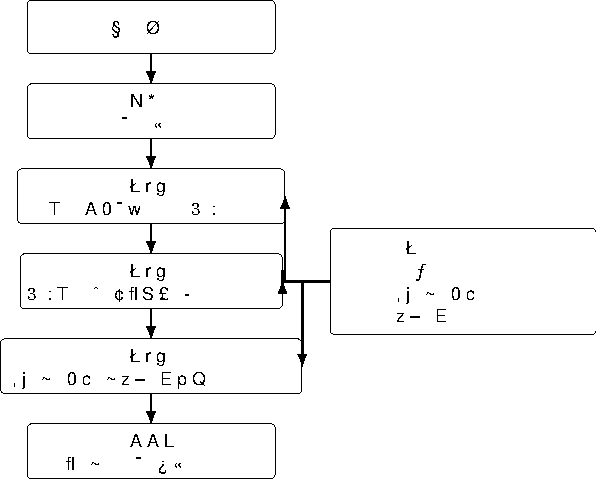
\includegraphics[width=0.94\columnwidth]{figure1.pdf}
\caption{想定するシステム構成．種目別設定を共通処理に入力し，設定で表現できない規則は個別処理へ拡張する．}
\label{fig:system}
\end{figure}
\par
設定データには，(a)角度計算に用いる3点のランドマーク名，(b)目標角度，(c)許容範囲，(d)比較条件を記述する．例えばスクワットなら「股関節・膝・足首」を指定し，膝角度90度，許容範囲$\pm15$度，比較条件を設定する．アームカールでは「肩・肘・手首」に変更するだけで，同じ角度計算・判定処理を利用することを狙う．つまり，本研究の中心はJSONという形式そのものではなく，\textbf{設定で表現する範囲，共通処理，個別処理の境界}である．
\par
一方，膝と股関節など複数角度を同時に満たす規則や，角度の変化・動作順序など時間的情報を使う規則は，3点と単一の許容範囲だけでは表現できない可能性がある．この場合，共通処理の拡張または種目固有の個別処理を追加する．「常に設定だけで種目追加する」のではなく，設定変更で対応できる範囲と，コードを追加すべき境界を明らかにすることが設計上の狙いである．

\section{実装}
実装にはPython，OpenCV，MediaPipeを用いる．OpenCVはカメラ映像の取得・画像処理，MediaPipe Pose Landmarkerは人体ランドマークの取得に利用する[4,5]．単一種目（スクワット）の試作では，Webカメラ映像の取得，姿勢推定，ランドマーク・骨格表示，3点からの膝角度計算，基準値との比較・判定，結果表示，JSONからの設定値読み込みまでを確認している．これは共通化方式そのものではなく，共通処理として利用する基本機能を確認した段階である．
\par
現在のコードでは，角度計算に用いる股関節・膝・足首がコードに固定されており，設定変更だけで対象関節を切り替えられる状態ではない．また，コードが参照する設定ファイルの場所や，判定に必要な\texttt{tolerance}等の項目も整備が必要である．したがって，\textbf{単一種目で確認済みの処理と，種目別設定を切り替える共通化部分は区別して扱う}．

\section{検証方法と考察の観点}
まず，3節の設計に基づき，設定形式（3点，目標角度，許容範囲，比較条件）と共通処理の範囲を確定した実装版を作る．スクワットとアームカールの設定を用意し，同一プログラムで意図した角度と判定結果が得られるかを確認する．既知の角度となる姿勢を用いて，算出角度が期待値と一致するか，設定条件に対する判定結果が期待どおりかを確認し，「設定変更だけで動く」と「正しく計算・判定できる」を分けて評価する．
\par
次に評価規則を段階的に追加する．(i)膝と肘のように関節指定だけが異なる規則，(ii)複数の角度・条件を組み合わせる規則，(iii)角度の変化や動作順序など時間的変化を用いる規則を対象とする．各追加を，(1)変更不要，(2)設定のみ変更，(3)共通コードの追加・変更，(4)種目固有の個別処理，に分類する．これにより，RQに対して設定だけで扱える範囲と，コードが必要になる境界を明らかにする．特に(3)と(4)を分け，共通処理を拡張すべき場合と種目固有の処理が必要な場合を区別する．
\par
変更量の削減を主張する場合は，種目ごとに個別実装した場合を比較対象とし，種目追加時の変更箇所や追加行数を，共通コード・個別処理・設定に分けて記録する．比較を行わない段階では削減量を断定せず，対応可能な評価規則と必要な変更内容を整理する．また，角度範囲内に入ったことは設定した評価基準に対する判定であり，それだけで「正しいフォーム」とは同一視しない．

検証対象とする評価規則は，単に種目数を増やすのではなく，必要となる処理の違いが分かるように選択する．例えば，スクワットの膝角度とアームカールの肘角度は，対象関節が異なるだけで，3点から角度を算出して閾値と比較するという構造が共通している．この場合に設定変更だけで動作すれば，関節指定を設定へ外部化する設計の有効性を確認できる．一方，膝角度と股関節角度を同時に満たす規則では，複数の特徴量をまとめて判定する仕組みが必要になる．さらに，立位から下降，底部，立位への遷移のように動作の順序を判定する場合には，複数フレームの情報を保持する必要がある．この違いを明示的に比較することで，「設定化できるか」を単純な種目数ではなく評価規則の性質から検討する．

\begin{table}[t]
\centering
\caption{検証する評価規則と想定する対応}
\small
\begin{tabular}{p{0.29\columnwidth}p{0.23\columnwidth}p{0.39\columnwidth}}
\toprule
規則 & 主な差異 & 検証する対応\\
\midrule
関節角度 & 対象3点 & 設定のみで変更\\
複数条件 & 複数角度 & 共通処理の拡張可否\\
時間的変化 & フレーム間の関係 & 個別処理等の必要性\\
\bottomrule
\end{tabular}
\end{table}

また，評価結果の正しさについては，設定した角度と実際に算出された角度を比較する．例えば，三点の幾何的な位置関係から90度になる姿勢を用意し，システムが90度付近を出力するかを確認する．続いて，目標90度，許容範囲$\pm15$度という設定に対し，75度，90度，105度など境界付近を含む入力を与え，判定結果が期待どおりになるかを確認する．これにより，「設定を読み込めた」ことだけでなく，設定値が特徴量計算と判定処理へ正しく反映されていることを確認する．

\section{考察の観点}
考察では，第一にRQに対する回答として，設定データだけで対応できた評価規則の範囲を整理する．第二に，設定だけでは不足した場合に，どの情報を追加すれば共通処理として扱えるのか，または個別処理として分離した方がよいのかを検討する．例えば，複数角度の条件を設定で表現できるように拡張する方法と，複雑な時間的規則を個別処理へ委ねる方法を比較し，設定の複雑化と共通化の範囲のバランスを考える．第三に，種目追加時の変更箇所を比較し，既存コードへの影響を抑えられたかを確認する．
\par
さらに，実装上の制約も記録する．姿勢推定ではカメラ位置や画像品質によってランドマークの精度が変化するため，本研究の「共通化できた」という結果は，姿勢推定そのものの精度を保証するものではない．また，設定ファイルに多くの例外条件を詰め込むと，設定だけで対応できても可読性や保守性が低下する可能性がある．したがって，設定項目を増やすこと自体を目的とせず，種目間で再利用できる処理を共通化し，種目固有の処理は明確に分離するという観点から設計結果を評価する．

\section{おわりに}
本研究では，カメラ映像から姿勢を推定してフォームを評価するシステムを複数種目へ拡張する際の実装・保守負担に着目し，種目別設定，共通処理，個別処理に分ける構成を設計した．現在はスクワットの単一種目試作で，映像取得から姿勢推定，角度計算，判定，表示，JSON読み込みまでを確認している．今後は設定ファイルとコードをそろえ，スクワットとアームカールを同一の共通処理で扱える実装を完成させる．その後，評価規則を段階的に増やし，設定変更だけで対応できる範囲，共通コードの変更が必要な範囲，個別処理が必要な範囲を明らかにする．

\begin{thebibliography}{9}
\small
\setlength{\itemsep}{0pt}
\bibitem{tanabe} 田邉英介，椋木雅之，高塚佳代子：運動過程をフィードバックする筋力トレーニング支援システム，2021年度電気・情報関係学会九州支部連合大会講演論文集，p.228，2021．
\bibitem{merca} C. Mercadal-Baudart, C. Liu, G. Farrell, M. Boyne, J. González Escribano, A. Smolic, C. Simms: Exercise quantification from single camera view markerless 3D pose estimation, Heliyon, Vol.10, No.6, e27596, 2024.
\bibitem{patidar} K. Patidar, M. A. Zaveri: Framework for Gym Posture Estimation Using MediaPipe and OpenCV, 2025 IEEE International Conference on Recent Advances in Computing and Systems (REACS), DOI: 10.1109/REACS67479.2025.11413297, 2025.
\bibitem{mediapipe} Google AI Edge: MediaPipe Pose Landmarker, \url{https://ai.google.dev/edge/mediapipe/solutions/vision/pose_landmarker}（参照 2026-09-21）．
\bibitem{opencv} OpenCV: OpenCV Documentation, \url{https://docs.opencv.org/4.x/}（参照 2026-09-21）．
\end{thebibliography}
\end{document}
